\chapter{Electronics}

CosmicWatches have to be mainly low-cost and easy to build. In order to achieve this, the components selected for the construction have been carefully curated to make sure these restrictions were met. This however might be greatly responsible for some of the odd features found while testing the detector, like the lack of linearity and fluctuations in amplification and peak-detected values of seemingly equal input signals. The full KiCad project can be found in the GitHub repository: \href{https://github.com/anvargasl/CosmicWatch-gamma-spectroscopy-PCB}{CosmicWatch-gamma-spectroscopy-PCB}. The component numbers shown in this chapter are the ones that would have to be placed on the PCB in order to recreate the example schematics.

\begin{figure}[H]
    \centering
    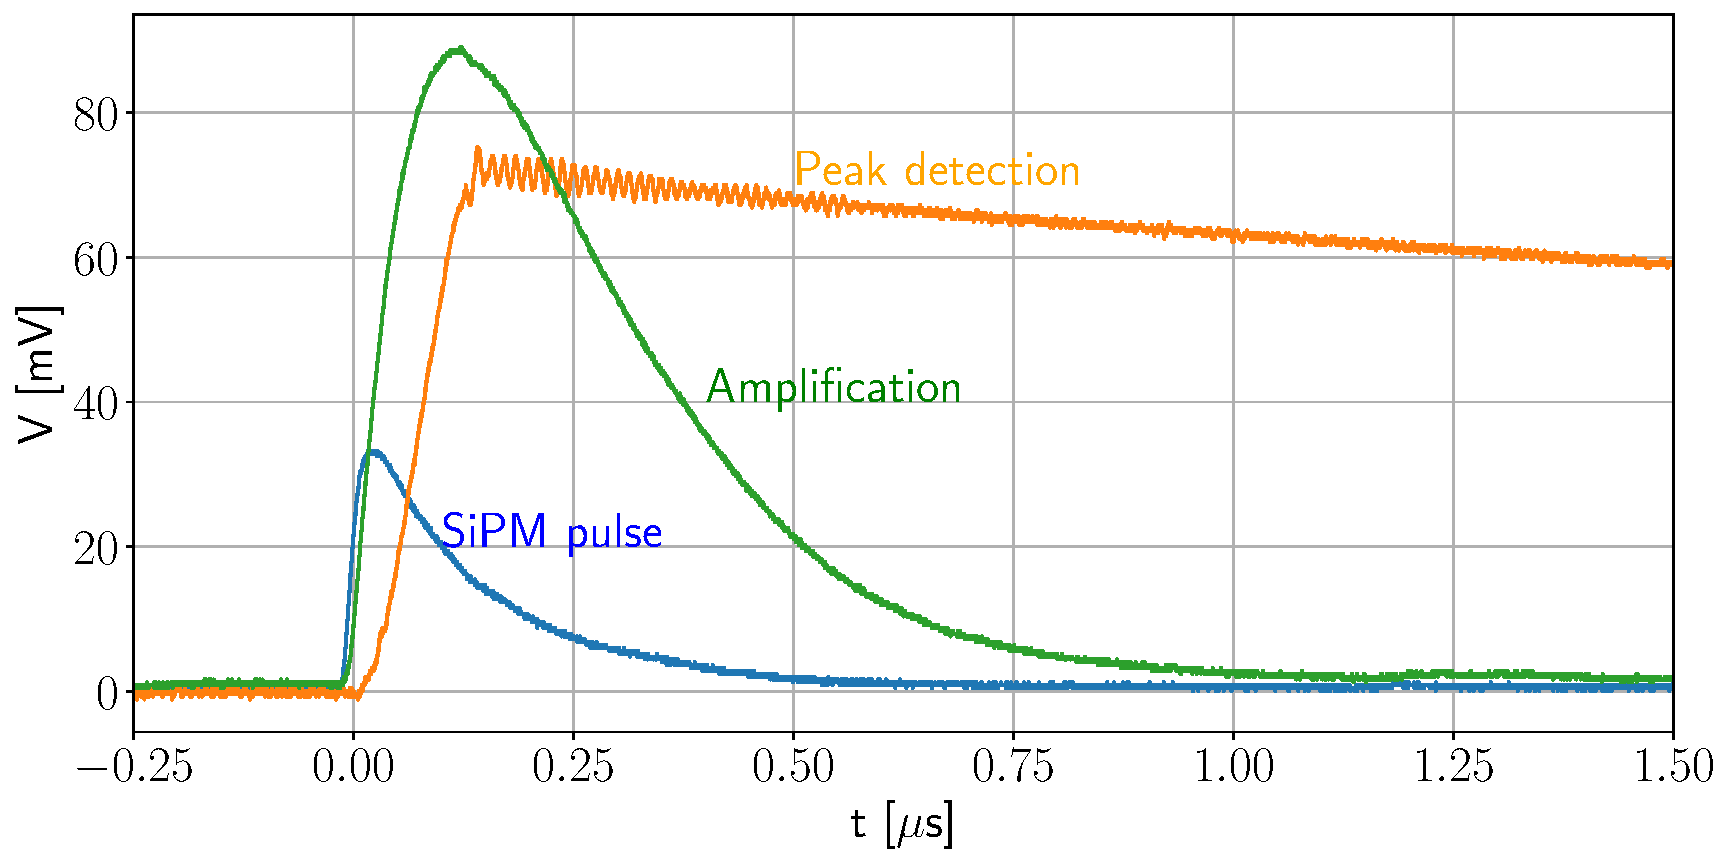
\includegraphics[width=0.8\textwidth]{Electronics/CW-signals.pdf}
    \caption{Signal processing inside the detector.}
    \label{fig:signal_processing}
\end{figure}

\section{Amplifier}

\begin{figure}[H]
    \centering
    \begin{circuitikz}[scale=0.7]
        \draw
        (0,0) node[op amp, noinv input up, font=\small] (opamp) {$U6$}
        (opamp.up) --++(0,0.5) node[vcc]{5\,\textnormal{V}}
        (opamp.down) --++(0,-0.5) node[vee]{-5\,\textnormal{V}}
        (opamp.+) node[left]{$V_{in}$}
        (opamp.-) node[left]{} to[short] ++(0, -3) coordinate(R4_R)
        to[R, l_=$R_4$] ++(-3, 0) node[ground]{}
        (R4_R) to[R, l_=$R_6$] ++(2.7, 0)
        %to[short] ++(0.1, 0) -|(opamp.out) to[short] ++(1, 0) node[ocirc, label={[yshift=0.3]$V_{out}$}]{}
        to[short] ++(0.1, 0) -|(opamp.out) to[short,-*] ++(1,0) node[above]{$V_{out}$};
        %to[short] ++(1, 0) node[ocirc, label=above:$V_{out}$]{};

        %Nodes
        %\node[shift={(0,+1.5)}] at (opamp) {U6 HLM6658};
    \end{circuitikz}
    \caption{Amplifier circuit schematic. An LT1807 op-amp is used for this and the peak detection stage.}
    \label{circ:amplifier}
\end{figure}

The processing of a pulse coming out of the SiPM has to go through two main stages, amplification and peak detection, Fig. \ref{fig:signal_processing} showcases these stages. The brightest SiPM pulses seen so far do not exceed 200 mV, which covers a very small portion of the ADC range on the RP Pico (0-3.3 V \cite[p.~18]{datasheet2024rp2040}). Amplification of the signal therefore allows for better resolution.

An op-amp on its own amplifies the voltage difference between the non-inverting (pin $+$) and inverting (pin $-$) inputs by its internal gain $A_{int}$, having then $V_{out}=A_{int}(V_+ - V_-)$. In this case, however, we are interested in controlling the gain of the circuit and therefore the amplification. In order to achieve this we introduce a feedback loop in the op-amp through $R4$ and $R6$, which controls how much of the output voltage is fed back into the op-amp. The theoretical amplification is therefore given by $V_{out}=(1+R6/R4)V_{in}$. A simple schematic showcasing the component arrangement is shown in Fig. \ref{circ:amplifier}.

\section{Peak Detector}

Since the LYSO crystal is so fast (36 ns of decay time \cite{Luxium_LYSO}) the ADC sample rate and response time of the Pico both play an important role in the number of events that the detector will accurately acquire. It is therefore necessary to hold the voltage of the amplified pulse in order to increase the chances of reading the actual value of the incoming signal. This is the task of the peak detector, to widen the time window in which we can sample the ADC and get a correct reading.

The idea behind the peak detector is to store charge in a capacitor ($C_{25}$) through a diode ($D_3$), retaining the highest voltage the input signal has reached. A diode is placed before the capacitor so that once the signal's voltage goes below the peak voltage, the diode will be reverse biased, therefore preventing current from flowing while maintaining the voltage on the capacitor.

In order to measure the voltage in the capacitor, a discharging resistor has to be added ($R_{15}/R_{19}$). The time it takes the capacitor to discharge is given by $t=RC$. Although for example in the case of CosmicWatch-V2's peak detector, the values of $R_{14}$ and $R_{24}$ also play a role in the discharging time, which has proved not to be as trivial as calculating the equivalent resistance $R_t$ of all three and simply take $t=R_tC$.

The schematic and PCB shown in the repository \href{https://github.com/anvargasl/CosmicWatch-gamma-spectroscopy-PCB}{CosmicWatch-gamma-spectroscopy-PCB}, include the connections and footprints necessary to place the components that make the designs illustrated in Subsections \labelcref{sec:basic,sec:pd_V2,sec:basic_buffer,sec:nuclear_phoenix}. Different results were found while testing these peak detector setups.

\subsection{Basic Peak Detector}\label{sec:basic}

\begin{figure}[H]
    \centering
    \begin{circuitikz}[scale=0.7]
        %\draw [help lines] (-4,0) grid (5,-4);
        \draw (0,0) node[op amp, noinv input up, font=\small] (opamp) {$U6$}
        (opamp.up) --++(0,0.5) node[vcc]{5\,\textnormal{V}}
        (opamp.down) --++(0,-0.5) node[vee]{-5\,\textnormal{V}}
        (opamp.+) node[left]{$V_{in}$}
        (opamp.out) node[]{} to[sD, l_=$D_3$] (6, 0) coordinate (D3_r)
        (opamp.-) node[left]{} to[short] ++(0, -2.5) coordinate (R24_l)
        (R24_l) to[R, l^=$R_{24}$, resistors/scale=0.8] (D3_r |- , |- R24_l) coordinate (R24_r)
        (D3_r) -- (R24_r)
        (D3_r) -- ++(1,0) coordinate (C25_u)
        (C25_u) to[C, l=$C_{25}$] ++(0,-2) node[ground]{}
        (C25_u) -- ++(2,0) to[R, l=$R_{15}$, resistors/scale=0.8] ++(0,-2) node[ground]{};
        %\draw (A |- 52,3)(D3_r) -- (R24_r);
        % to[short] ++(-0.1, 0) -|(R24_r)
    \end{circuitikz}
    \caption{Basic peak detector design.}
    \label{circ:basic_pd}
\end{figure}

Assuming ideal conditions, a diode is enough to retain the highest input voltage reached. Semiconductor diodes however don't behave ideally, they introduce a voltage drop that will keep the voltage stored in $C_{25}$ at a lower potential than that of $V_{in}$. In order to prevent this, an op-amp $(U_6)$\footnote{Currently the only op-amp that has behaved reasonably well is the LT1807 by Analog Devices Inc. The LMH6658  by Texas Instruments seems to have trouble driving even small capacitors.} is placed before the diode. In the configuration shown in Fig. \ref{circ:basic_pd}, the opamp will try to output the necessary current to equilibrate the inverting input voltage (pin $-$) to what it sees in the non-inverting input (pin $+$), to achieve this $U_6$ has to go one diode drop above $V_{in}$.

\subsection{Preventing negative saturation}\label{sec:pd_V2}

\begin{figure}[H]
    \centering
    \begin{circuitikz}[scale=0.7]
        %\draw [help lines] (-4,0) grid (5,-4);
        \draw (0,0) node[op amp, noinv input up, font=\small] (opamp) {$U_6$}
        (opamp.up) --++(0,0.5) node[vcc]{5\,\textnormal{V}}
        (opamp.down) --++(0,-0.5) node[vee]{-5\,\textnormal{V}}
        (opamp.+) node[left]{$V_{in}$}
        (opamp.out) -- ++(1,0) coordinate(oa_out) to[sD, l_=$D_3$] (6, 0) coordinate (D3_r)
        (opamp.-) -- ++(0, -2.7) coordinate (ver_1) -- ++(1, 0) coordinate(D5_l)
        (ver_1) to[R, l_=$R_{14}$, resistors/scale=0.8] ++(-2,0) node[ground]{} 
        (D5_l) to[sD, l_=$D_5$] (oa_out |- , |- D5_l) coordinate (D5_r)
        (oa_out) -- (D5_r)
        (D5_l) -- ++(0,-1.7) coordinate (R24_l)
        (R24_l) to[R, l^=$R_{24}$, resistors/scale=0.8] (D3_r |- , |- R24_l) coordinate (R24_r)
        (D3_r) -- (R24_r)
        (D3_r) -- ++(1,0) coordinate (C25_u)
        (C25_u) to[C, l=$C_{25}$] ++(0,-2) node[ground]{}
        (C25_u) -- ++(2,0) to[R, l=$R_{15}$, resistors/scale=0.8] ++(0,-2) node[ground]{};
    \end{circuitikz}
    \caption{Basic peak detector design, a second diode is added in order to prevent the op-amp from entering a negative saturation loop.}
    \label{circ:pd_V2}
\end{figure}

In the basic peak detector, once the signal voltage goes below the peak voltage, $D_3$ will be reverse biased and the inverting input of the opamp will see a higher voltage than the non-inverting input, this will force $U_6$ to go into negative saturation by driving the output voltage as low as it can in order to match both inputs. Once the signal gets close to the stored voltage in $C_25$, the op-amp will have to get out of the negative saturation, this will take some time which depends on the slew rate of the opamp and therefore limits the operating frequency range of the circuit.

In order to avoid negative saturation $D_5$ is added, along with an outer feedback loop through $R_{24}$. In this case, once the input signal goes below the stored voltage, $D_5$ will be forward biased, allowing for a new feedback loop that decreases the op-amp's negative saturation time.


\subsection{Basic Peak Detector + Buffer}\label{sec:basic_buffer}

\begin{figure}[H]
    \centering
    \begin{circuitikz}[scale=0.7]
        %\draw [help lines] (-4,0) grid (5,-4);
        \draw (0,0) node[op amp, noinv input up, font=\small] (opamp) {$U_6$}
        (opamp.up) --++(0,0.5) node[vcc]{5\,\textnormal{V}}
        (opamp.down) --++(0,-0.5) node[vee]{-5\,\textnormal{V}}
        (opamp.+) node[left]{$V_{in}$}
        (opamp.out) -- ++(1,0) coordinate(oa_out) to[sD, l_=$D_3$] (6, 0) coordinate (D3_r)
        (opamp.-) -- ++(0, -2.7) coordinate (ver_1) -- ++(1, 0) coordinate(D5_l)
        (ver_1) to[R, l_=$R_{14}$, resistors/scale=0.8] ++(-2,0) node[ground]{} 
        (D5_l) to[sD, l_=$D_5$] (oa_out |- , |- D5_l) coordinate (D5_r)
        (oa_out) -- (D5_r)
        (D5_l) -- ++(0,-1.7) coordinate (R24_l)
        (D3_r) -- ++(1,0) coordinate (C25_u)
        (C25_u) to[C, l=$C_{25}$] ++(0,-2) node[ground]{}
        (C25_u) -- ++(2,0) coordinate (buffer_l)
        (buffer_l) node[op amp, noinv input up, font=\small, anchor=+] (buffer) {$U_7$}
        (buffer.-) coordinate (buffer_-)
        (buffer.out) coordinate (buffer_out)
        (buffer_-) -- (buffer_- |-, |- R24_l) coordinate (R24_r)
        (R24_l) to[R, l^=$R_{24}$, resistors/scale=0.8] (R24_r)
        (R24_r) -- (buffer_out |-, |- R24_r) -- (buffer_out)
        (buffer_out) to[short, -*] ++(1,0);
        %(D3_r) -- (R24_r);
        %(C25_u) -- ++(2,0) to[R, l=$R_{15}$, resistors/scale=0.8] ++(0,-2) node[ground]{};
    \end{circuitikz}
    \caption{Basic peak detector design, Adding a buffer to prevent discharging of the capacitor through the resistor and instead through any load in the circuit, in this case $R_29$.}
    \label{circ:pd_buffer}
\end{figure}

This design follows the same principles as the one shown in the previous subsection. However, in this case, a buffer is added to introduce high impedance and prevent the capacitor from discharging through the resistor and instead through any load that may be applied after the circuit.

\subsection{Nuclear Phoenix}\label{sec:nuclear_phoenix}

\begin{figure}[H]
    \centering
    \begin{circuitikz}[scale=0.7]
        %\draw [help lines] (-4,0) grid (5,-4);
        \draw (0,0) node[op amp, noinv input up, font=\small] (opamp) {$U_6$}
        (opamp.up) --++(0,0.5) node[vcc]{5\,\textnormal{V}}
        (opamp.down) --++(0,-0.5) node[vee]{-5\,\textnormal{V}}
        (opamp.+) node[left]{$V_{in}$}
        (opamp.out) coordinate(oa_out) to[sD, l_=$D_5$] ++(2, 0) coordinate (D5_r)
        (D5_r) to[sD, l_=$D_3$] ++(2, 0) coordinate (D3_r)
        (D5_r) -- ++(0,-4) coordinate (R30_l)
        (D3_r) -- ++(3,0) coordinate (C25_u)
        (C25_u) to[C, l=$C_{25}$] ++(0,-2) node[ground]{}
        (C25_u) -- ++(2,0) coordinate (buffer_l)
        (opamp.-) coordinate (oa_-)
        (oa_-) -- ++(-1.5, 0) -- ++(0, 4) coordinate(aux1)
        (aux1) -- (D3_r |-, |- aux1) -- (D3_r)
        (buffer_l) node[op amp, noinv input up, font=\small, anchor=+] (buffer) {$U_7$}
        (buffer.-) coordinate (buffer_-)
        (buffer.out) coordinate (buffer_out)
        (buffer_-) -- (buffer_- |-, |- R30_l) coordinate (R30_r)
        (R30_l) to[R, l_=$R_{30}$, resistors/scale=0.8] (R30_r)
        (R30_r) -- (buffer_out |-, |- R30_r) -- (buffer_out)
        (buffer_out) to[short, -*] ++(1,0);
        %(D3_r) -- (R24_r);
        %(C25_u) -- ++(2,0) to[R, l=$R_{15}$, resistors/scale=0.8] ++(0,-2) node[ground]{};
    \end{circuitikz}
    \caption{Nuclear Phoenix peak-detector design. Taken from \cite{Nucelar_phoenix}.}
    \label{circ:pd_np}
\end{figure}

NuclearPhoenix is a physics student who has developed a gamma detector that also utilizes a Raspberry Pi Pico and a Silicon photomultiplier, his schematics also include a peak detection circuit which is shown in Fig. \ref{circ:pd_np}, his project can be found in \href{https://nuclearphoenix.xyz/hardware/ogd/}{Open Gamma Detector}. This design aims to prevent leakage current across $D_3$, this discharges the capacitor at a faster rate than intended once the peak voltage has been reached. In this case, $R_30$ is feeding back the peak voltage value to $D_3$, therefore creating a 0 V difference across the diode, preventing any leakage current from flowing out of $C_{25}$ and into the output of the op-amp.

\section{Trigger}

\begin{figure}[H]
    \centering
    \begin{circuitikz}[scale=0.7]
        %\draw [help lines] (-4,0) grid (5,-4);
        \draw (0,0) node[op amp, noinv input up, font=\small] (opamp) {$U_6$}
        (opamp.up) --++(0,0.5) node[vcc]{5\,\textnormal{V}}
        (opamp.down) --++(0,-0.5) node[vee]{-5\,\textnormal{V}}
        (opamp.out) --++(1,0) node[above]{$V_{out}$}
        (opamp.+) node[left]{$V_{in}$}
        (opamp.-) --++(-2.5,0)  coordinate (oa_-)
        (oa_-) to[R, l^=$R_{16}$, resistors/scale=0.8] ++(0,2) to[R, l^=$R_{22}$, resistors/scale=0.8] ++(0,2) node[vcc]{5\,\textnormal{V}}
        (oa_-) to[R, l_=$R_{18}$, resistors/scale=0.8] ++(0,-2) node[ground]{};

        %Nodes
        \node[shift={(-0.3,-0.3)}] at (opamp.-) {$V_{REF}$};
    \end{circuitikz}
    \caption{Trigger circuit.}
    \label{circ:trigger}
\end{figure}

In this case, a voltage divider is used to force a positive saturation in the op-amp once the amplified signal reaches a threshold voltage, generating a "digital 1"\: that can be used to trigger the detector. The threshold, or $V_{REF}$ as noted in Fig. \ref{circ:trigger}, is given by equation \eqref{eq:v_ref}.

\begin{equation}
    V_{REF}=\frac{R_{18}}{R_{22}+R_{16}+R_{18}} V_{cc} \label{eq:v_ref}
\end{equation}

%add code as appendix
\section{Microcontroller}

\section{DC to DC booster}

\begin{figure}[H]
    \centering
    \begin{circuitikz}
        % U1 NE555
        \draw [thick] (0,0) coordinate (u1) rectangle ++(2,3); % shape
        \draw [pin] (u1) ++(1, 3.8)
            node[]{$U_1$};
        \draw [pin] (u1) ++(1, 3.3)
            node[]{MAX5026};
        %-----------Left side-----------%
        \draw [pin] (u1) ++ (0,2.5) coordinate (u1 pgnd)
            node[right, font=\scriptsize]{PGND}
            node[above left]{1}; % CON
        \draw [pin] (u1) ++ (0,1.5) coordinate (u1 gnd)
            node[right, font=\scriptsize]{GND}
            node[above left]{2}; % TRI
        \draw [pin] (u1) ++ (0,0.5) coordinate (u1 fb)
            node[right, font=\scriptsize]{FB}
            node[above left]{3}; % THR
        
        %-----------Right side-----------%
        \draw [pin] (u1) ++ (2,2.5) coordinate (u1 lx)
            node[left, font=\scriptsize]{LX}
            node[above right]{6}; % OUT
        \draw [pin] (u1) ++ (2,1.5) coordinate (u1 vcc)
            node[left, font=\scriptsize]{VCC}
            node[above right]{5}; % OUT
        \draw [pin] (u1) ++ (2,0.5) coordinate (u1 shdn)
            node[left, font=\scriptsize]{SHDN}
            node[above right]{4}; % OUT
        %\draw (u1) ++ (2,0)
        %    node[right]{\ctikzlabel{$U_1$}{NE555}}; % NE555P
        
        % U1 NE555 Pins
        \draw (u1 pgnd) -- ++ (-1,0) node[ground]{}; % PGND

        \draw (u1 gnd) -- ++ (-1,0) node[ground]{}; % GND

        \draw (u1 fb) -- ++ (-2,0) coordinate(r10 u) to[R, l_=$R_{10}$, resistors/scale=0.8] ++(0,-2) node[ground]{}
        (r10 u) to[R, l^=$R_{2}$, resistors/scale=0.8] ++(0,2) -- ++(0,2) -- ++(7,0) coordinate(d4 r)
        (d4 r) --++(2,0) coordinate(c3 u) to[R, l^=$R_{25}$, resistors/scale=0.8] ++(2,0) coordinate (c4 u)
        (c3 u) to[C, l_=$C_{3}$, resistors/scale=0.8] ++(0,-2)  node[ground]{}
        (c4 u) to[C, l_=$C_{4}$, resistors/scale=0.8] ++(0,-2)  node[ground]{}
        (c4 u) --++(1,0) node[vcc]{\textnormal{HV}}; % FB

        \draw (u1 lx) -- ++ (1,0) coordinate(d4 l)
        (d4 l) -- ++(0,1) to[sD, l^=$D_3$] ($(d4 r) + (0,-1)$) -- (d4 r)
        (d4 l) to[american inductor, l_=$L_1$] ($(d4 r) + (0,-2)$) coordinate(l1 r); % LX

        \draw (u1 vcc) -- ++ (1,0) to[short, -*] ++(0,-1); % VCC

        \draw (u1 shdn) --++(2,0) coordinate(c7 u) --++(1,0) coordinate (c2 u) --(l1 r)
        (c7 u) to[C, l_=$C_{7}$, resistors/scale=0.8] ++(0,-2) node[ground]{}
        (c2 u) to[C, l=$C_{2}$, resistors/scale=0.8] ++(0,-2) node[ground]{}
        (c2 u) --++(1,0) node[vcc]{5\,\textnormal{V}}; % SHDN
    \end{circuitikz}
    \caption{DC to DC booster circuit. Careful considerations have to be made when placing the MAX5026 IC in order to reduce noise on the power line. It is advised to have a look at the datasheet in \cite{AnalogDevices_DC_DC}, section "Applications Information".}
    \label{circ:booster}
\end{figure}

Acording to Onsemi \cite{Onsemi_SiPM}, the operaing voltage of a MicroFJ-300XX-TSV SiPM is 25.2-30.7 V. It is then necessary to boost $V_{cc}$ to the operating range of the SiPM, noted as HV in Fig. \ref{circ:booster}. In order to achive this, a MAX5026 PWM Step-Up DC-DC Converter is used \cite{AnalogDevices_DC_DC}, which has a user-adjustable output voltage of up to 36 V using external feedback resistors.

In the circuit shown in Fig. \ref{circ:booster}, $R_{10}$ and $R_2$ determine the output voltage HV. According to \cite{AnalogDevices_DC_DC}, equation \eqref{eq:booster_fb_resistance} allows to calculate the Value of $R_{10}$ given a desired output voltage HV and a value of $R_2$ between 5 and 50 \unit{\kilo\ohm}.

\begin{equation}
    R_{10} = R_2\left(\frac{\text{HV}}{V_{REF}}-1\right) \label{eq:booster_fb_resistance}
\end{equation}

\section{Single photons}